\section{Finding the Right Prices}


The question remains: What is the right price? Should we average the
\(l^{(j)}_i\) somehow?

It turns out, that ensuring supply to be equal to demand
\(S=D\) leaves us with very little choice when it comes to prices anyway.
Let us see what happens for a fixed price vector. We want \(S=D\). This
obviously implies
\begin{equation}
	\label{eq: supply gdp = demand gdp}
	0 =\langle S-D,p\rangle =  \sum_{i=1}^n \langle S_i - D_i, p\rangle
\end{equation}
A market based system on the other hand ensures
\[
	0 = \langle S_i - D_i, p\rangle
	= \underbrace{\langle S_i, p\rangle}_{\text{income}}
	- \underbrace{\langle D_i,p\rangle}_{\text{expenses}}
\]
which is more than sufficient for the sums in Equation~\eqref{eq: supply gdp =
demand gdp} to be equal, but not sufficient for \(S=D\). In fact, it only
ensures that the price is orthogonal to the demand/supply mismatch \(S-D\).
If there are \(d\) products, that leaves a \(d-1\) hyperplane.

But as we will see, there are some price vectors, which do ensure \(S=D\).
We call these economic equilibria.

\begin{figure}
	\centering
	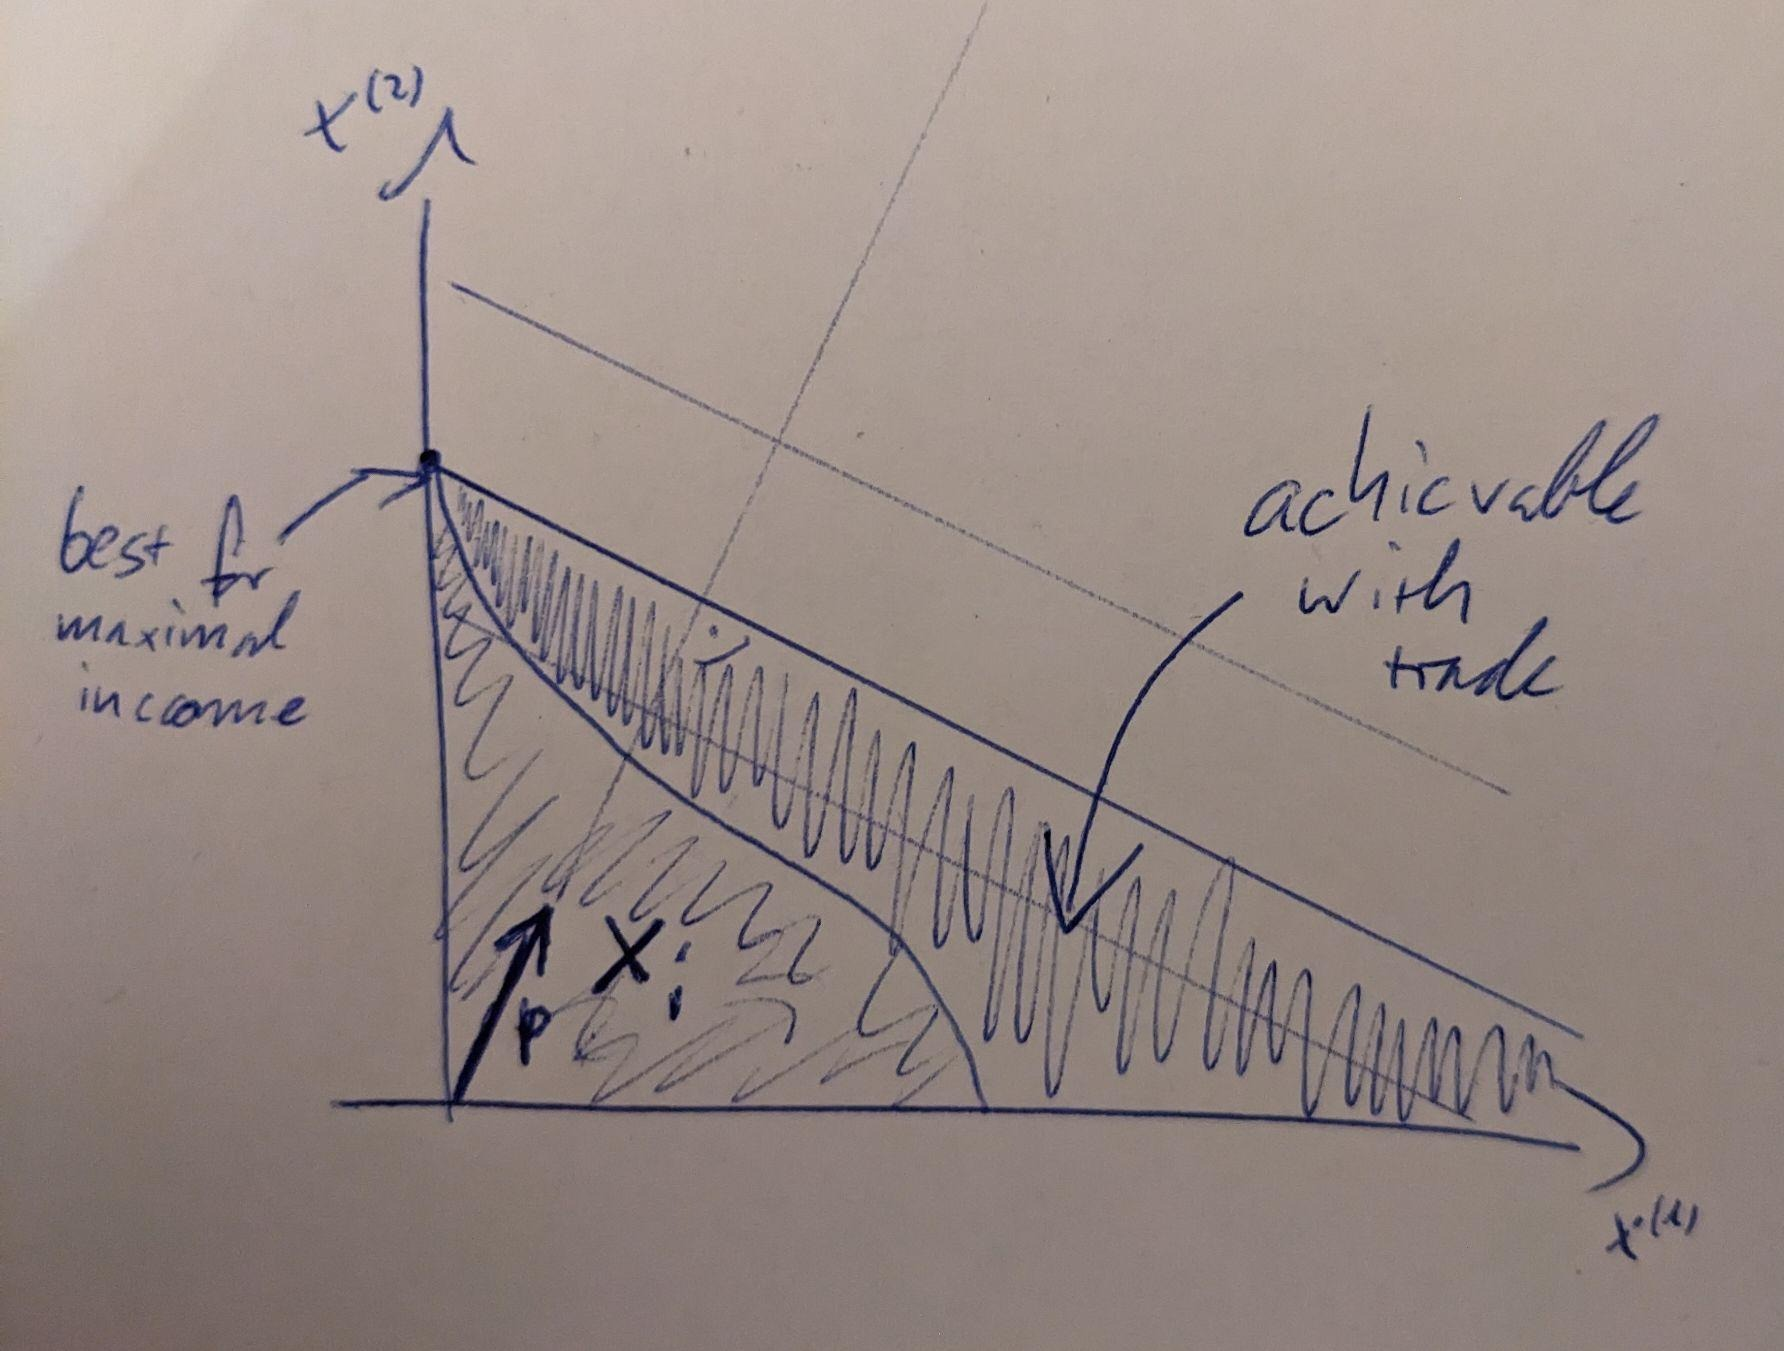
\includegraphics[width=0.7\textwidth]{images/consumption_increase_by_trade.jpeg}
	\caption{
		Product vectors on the \(d-1\) dimensional hyperplanes orthogonal to \(p\)
		cost the same amount and can therefore be exchanged (here \(d=2\), so the
		hyperplanes are lines). Trading at prices \(p\) enlarges the set of
		product vectors available for consumption for person \(i\).
	}
	\label{fig: consumption increase by trade}
\end{figure}
For a fixed price vector \(p\), let us consider the production and consumption
decision of person \(i\). As their expenses have to be smaller than their
income, it makes sense to maximize income for a given amount of labour \(L_i\).
Recall that our production options are \(X_i=X_i(L_i)\). So the maximal income
given labour \(L_i\) is
\[
	\tag{income}\label{eq: income}
	\mu(p, X_i) := \sup\{\langle p, x\rangle : x\in X_i\}.
\]
The function \(\mu(\cdot, X_i)\) in \(p\), is called the ``support function'' of
\(X_i\). It has some useful properties we will be grateful for later on. The
individual decision problem of person \(i\) therefore becomes
\begin{equation}
	\tag{IDP}
	\label{eq: individual decision problem}
	\max_{L_i, y} u(1-L_i, y) \quad\text{subject to}\quad \langle y, p\rangle \le \mu(p, X_i(L_i))
\end{equation}
In Figure~\ref{fig: consumption increase by trade} we can see, how this
constraint is always weaker than \(y\in X_i(L_i)\), which is the constraint of
self-sufficiency. I.e. we get the following lemma.

\begin{lemma}[Trade is never harmful]
\[
	\underbrace{X_i(L_i)}_{\text{own production}}
	\subseteq \quad
	\underbrace{
		\{y\in\real_{\ge 0}^\dims: \langle y, p\rangle \le \mu(p, X_i)\}
	}_{\text{consumption options with trade}}
\]
\end{lemma}
\begin{proof}
	Choose an arbitrary \(y\in X_i\), then by definition of \(\mu\)
	\[
		\langle p, y\rangle \overset{y\in X_i}\le \sup\{\langle p, x\rangle : x\in
		X_i\} \overset{\text{def.}}= \mu(p, X_i),
	\]
	\(y\) is also in the set on the right.
\end{proof}

\subsection{Supply and Demand}

Before we move on, let us quickly define supply and demand. The demand of
individual \(i\) is given by
\[
	D_i(p) := \{
		y : (L,y)
		\text{ is a solution to \eqref{eq: individual decision problem}}
	\}.
\]
Notice that it is a set, since there might be multiple solutions. The same is
true for the supply of individual \(i\)
\[
	S_i(p) := \argmax_{x\in X_i} \langle p, x\rangle 
	\overset{(*)}= \nabla_p \mu(p, X_i).
\]
Where \((*)\) is a property of the support function \(\mu(\cdot,
X_i)\)\fxnote{source or explanation}.
We can then define total demand and supply
\[
	D(p) := \sum_{i=1}^n D_i(p),
	\qquad
	S(p) := \sum_{i=1}^n S_i(p),
\]
where the sums are Minkowski sums\footnote{
	The Minkowski sum of set \(A\) and \(B\) is defined as
	\[
		A + B := \{ x+y : x\in A, y\in B\}
	\]
}.
And \(p^*\) is a market equilibrium, if
\[
	S(p^*)\cap D(p^*)\neq\emptyset.
\]
If \(S(p^*)\) and \(D(p^*)\) only contain a single element, one may write
\(S(p^*)=D(p^*)\).

\begin{lemma}[Income in the Pure Variable Cost Case]
	In the pure variable cost case \(L_i(x) = \langle l_i, x\rangle\), income
	can be written as
	\[
		\mu(p, X_i(L_i))
		= \overbrace{L_i}^{\text{work time}} \max_{j=1,\dots,\dims}
		\underbrace{\frac{p_j}{l_i^{(j)}}}_{=: w_i^{(j)}}
		= L_i \overbrace{\|w_i\|_\infty}^{\text{wage}},
	\]
	where \(w_i^{(j)}\) are potential wages for producing good \(j\).
\end{lemma}
\begin{proof}
	Let \(H:= \diag(l_i)\), then as \(X_i\) is compact we know the supremum is
	a maximum and
	\begin{align*}
		\mu(p, X_i)
		&= \max_{x\ge 0} \langle p, x\rangle
		\text{ s.t. } \langle x, l_i\rangle \le L_i\\
		&\overset{y=Hx}= \max_{y\ge 0} \langle p, H^{-1}y\rangle
		\text{ s.t. } \underbrace{\langle H^{-1}y, l_i\rangle}_{
			= \langle y, 1 \rangle = \|y\|_1
		} \le L_i\\
		&= L_i \underbrace{
			\max_{y\ge 0} \langle H^{-1}p, y\rangle \text{ s.t. } \|y\|_1 \le 1
		}_{
			= \|H^{-1} p\|_{\text{Op-Norm(1)}} = \|H^{-1} p \|_\infty
		}\\
		&= L_i \max_{j=1,\dots,\dims} \frac{p_j}{l_i^{(j)}},
	\end{align*}
	where we have used, that all entries of \(y\) are non-negative when
	converting to the \(1\)-norm, \(\|x\|_1 = \sum_{i=1}^\dims |x_i|\), the
	fact that the operator norm of the \(1\)-norm is the sup norm
	\(\|x\|_\infty = \sup_{i=1,\dots,\dims} |x_i|\)\fxnote{source or appendix},
	and finally positivity of entries of \(p\) and \(l_i\) again.
\end{proof}

\begin{example*}[Pure Variable Cost Case]
	The individual decision problem \eqref{eq: individual decision problem}
	therefore becomes
	\[
		\max_{L_i, y} u(1-L_i, y) \text{ s.t. } \langle p, y\rangle \le L_i \|w_i\|_\infty
	\]
	or in other words
	\[
		\max_{y} u\left(1- \frac{\langle p, y\rangle}{\|w_i\|_\infty}, y\right).
	\]
	The first order condition is therefore
	\[
		\frac{du}{dy} 
		= u_f\Bigl[
			\underbrace{\frac{u_y}{u_f}}_{\text{wtw}}
			- \overbrace{\frac{p}{\|w_i\|_\infty}}^{\text{effort required}}
		\Bigr]
		= \frac{u_f}{\|w_i\|_\infty}\Bigl[
			\underbrace{\frac{u_y}{u_f}\|w_i\|_\infty}_{\text{wtp}}
			- p
		\Bigr]
	\]
	Where the ``willingness to pay'' (wtp) is simply the willingness to work
	(wtw) scaled by person \(i\)'s wages.
	
\end{example*}


\subsection{Cloned Hermit Economy}

In this subsection we are going to consider economies consisting of identical
clones, to build intuition for the real deal.

\begin{example*}[Pure Variable Cost]

\end{example*}

In the example above, trade did not offer an improvement over the lone hermit
case. This is the case for convex \(X_i\) in general.
Let us consider the case of concave production capabilities \(X_i\).

\begin{figure}
	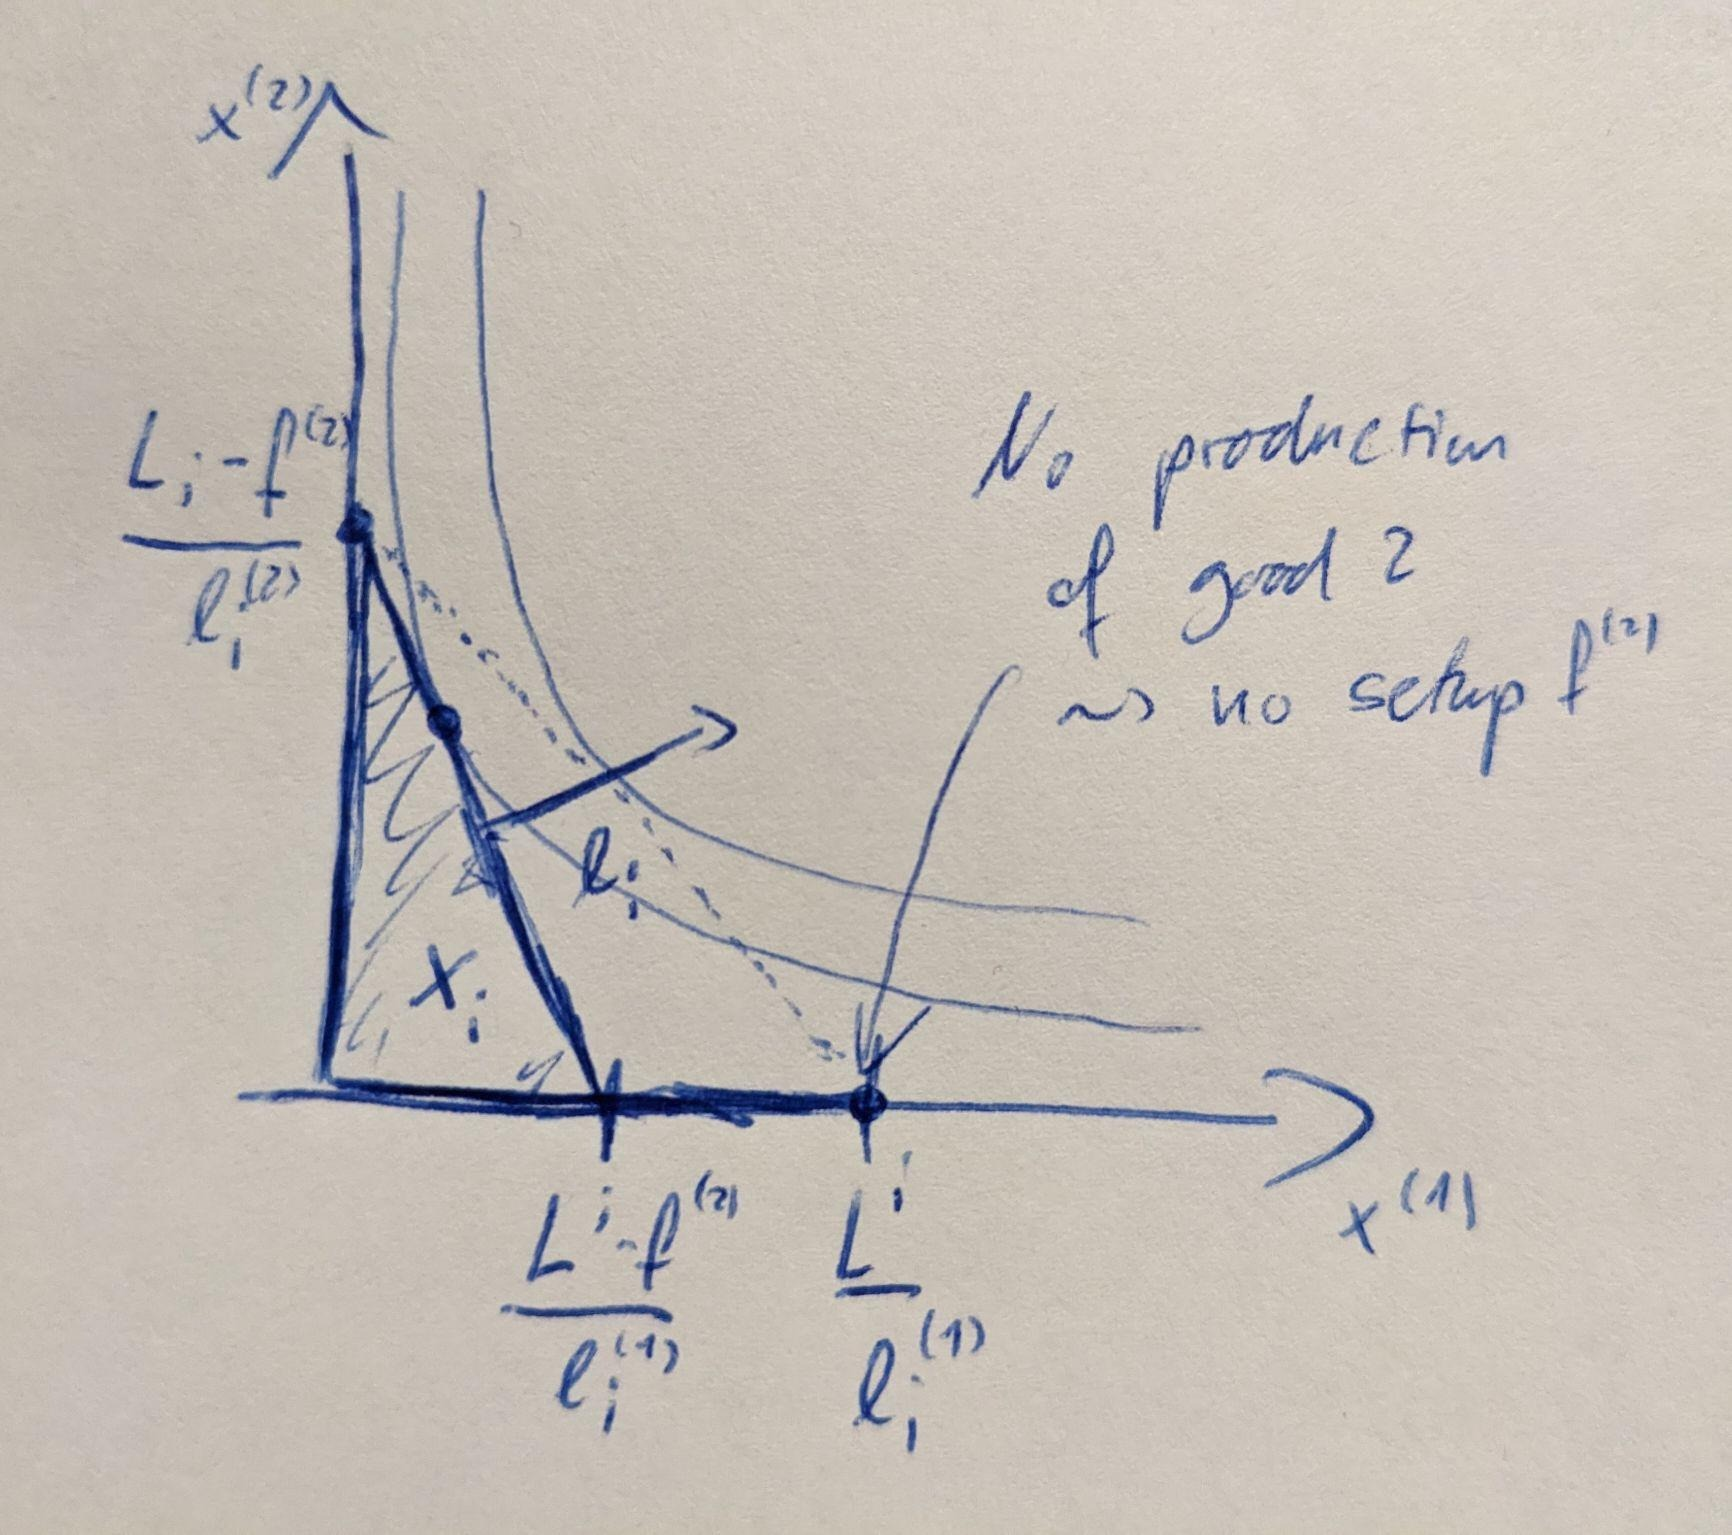
\includegraphics[width=0.58\textwidth]{images/hermit-decision-setup-cost.jpeg}
	\caption{
	fixed set-up time \(f^{(2)}\) for the production of good \(2\). This allows
	for more production of good \(1\) if \(x^{(2)}=0\). The dotted line
	represents the production frontier in the ``cloned hermit economy''.}
\end{figure}